\section{Le repère}

Ces macros remplacent celles de \tkzname{tkz-base} (\tkzcname{tkzInit}, \tkzcname{tkzGrid}, \tkzcname{tkzAxeXY}, \tkzcname{tkzDrawX}, \tkzcname{tkzClip}, \tkzcname{tkzRep}, \tkzcname{tkzText}).

\subsection{Initialisation : \tkzcname{tkzFnInit}}

\begin{NewMacroBox}{tkzFnInit}{\oarg{options}}
\begin{tabular}{lll}
\toprule
options             & défaut & définition  \\
\midrule
\TOline{xmin}{-5}{plus petite abscisse}
\TOline{xmax}{5}{plus grande abscisse}
\TOline{xstep}{1}{valeur représentée par 1 cm sur l'axe des abscisses}
\TOline{ymin}{-5}{plus petite ordonnée}
\TOline{ymax}{5}{plus grande ordonnée}
\TOline{ystep}{1}{valeur représentée par 1 cm sur l'axe des ordonnées}
\TOline{xorigin}{0}{abscisse placée en $X=0$ (par exemple une année)}
\TOline{yorigin}{0}{ordonnée placée en $Y=0$}
\TOline{enlarge}{0 (0.1 sans valeur)}{élargit la fenêtre d'une fraction de sa taille}
\TOline{enlarge x, enlarge y}{enlarge}{élargissement dans une seule direction}
\bottomrule
\end{tabular}

\emph{Les valeurs peuvent être des expressions : \texttt{xmax=2*pi}.}
\end{NewMacroBox}

\subsection{Grille : \tkzcname{tkzFnGrid}}

\begin{NewMacroBox}{tkzFnGrid}{\oarg{options}\parg{$x_1$,$y_1$}\parg{$x_2$,$y_2$}}
\emph{La région est facultative ; par défaut la grille couvre la fenêtre.}

\begin{tabular}{lll}
\toprule
options             & défaut & définition  \\
\midrule
\TOline{dx}{xstep}{écart entre deux lignes verticales}
\TOline{dy}{ystep}{écart entre deux lignes horizontales}
\TOline{sub}{false}{ajoute une sous-grille}
\TOline{subdx}{dx/5}{écart de la sous-grille}
\TOline{subdy}{dy/5}{écart de la sous-grille}
\bottomrule
\end{tabular}

\emph{Les autres options sont celles de \TIKZ ; le style est \tkzname{tkzfn grid}.}
\end{NewMacroBox}

\begin{tkzexample}[latex=8cm]
\begin{tikzpicture}[scale=1.25]
 \tkzFnInit[xmin=-2,xmax=3,
            ymin=-1,ymax=2]
 \tkzFnGrid[sub,color=orange]
 \tkzFnAxes
\end{tikzpicture}
\end{tkzexample}

\subsection{Axes : \tkzcname{tkzFnAxes}, \tkzcname{tkzFnAxisX}, \tkzcname{tkzFnAxisY}}

\begin{NewMacroBox}{tkzFnAxes}{\oarg{options}}
\emph{Trace les deux axes, les graduations et leurs valeurs. Les axes se coupent en $(0~;~0)$ si ce point est dans la fenêtre, sinon en $(x_{\min}~;~y_{\min})$. Les valeurs sont écrites sous la forme française ou américaine (section~\ref{sec:format}).}

\begin{tabular}{lll}
\toprule
options             & défaut & définition  \\
\midrule
\TOline{dx, dy}{xstep, ystep}{écart entre deux graduations}
\TOline{xlabel, ylabel}{\$x\$, \$y\$}{noms des axes}
\TOline{ticks}{true}{graduations}
\TOline{labels}{true}{valeurs des graduations}
\TOline{line}{true}{tracé des axes}
\TOline{origin}{O ou 0}{nom de l'origine (O en français, 0 en américain)}
\TOline{trig}{0}{si $n>0$, graduations de l'axe des abscisses en multiples de $\pi/n$}
\TOline{decimals}{4}{nombre maximum de décimales}
\TOline{box}{false}{présentation « boîte » (section~\ref{sec:box})}
\TOline{style}{school}{\texttt{school} ou \texttt{box}}
\TOline{tick length}{3pt}{longueur des graduations (boîte)}
\TOline{arrows}{end}{flèches : \texttt{end}, \texttt{both} (aux deux extrémités) ou \texttt{none}}
\bottomrule
\end{tabular}

\emph{\tkzcname{tkzFnAxisX} et \tkzcname{tkzFnAxisY} tracent un seul axe ; leurs options sont les mêmes avec \tkzname{label}, \tkzname{label style} et \tkzname{step} à la place de \tkzname{xlabel}, \tkzname{ylabel} et \tkzname{dx}. Avec \tkzname{ticks=false}, on obtient l'équivalent de \tkzcname{tkzDrawX}.}
\end{NewMacroBox}

\begin{tkzexample}[latex=8cm]
\begin{tikzpicture}
  \tkzFnInit[xmin=-7,xmax=7,
             ymin=-1,ymax=1]
  \tkzFnAxisY
  \tkzFnAxisX[trig=2]
  \tkzFnDraw[red]{sin(x)}
\end{tikzpicture}
\end{tkzexample}

\subsection{Découpage : \tkzcname{tkzFnClip}}

\begin{NewMacroBox}{tkzFnClip}{\oarg{marge en pt}}
\emph{Restreint la suite du dessin à la fenêtre du repère (agrandie d'une marge). Comme \tkzcname{clip}, on l'utilise de préférence dans un environnement \tkzname{scope}. Les courbes et les tangentes sont de toute façon découpées à la fenêtre (option \tkzname{clip}).}
\end{NewMacroBox}

\subsection{Vecteurs du repère : \tkzcname{tkzFnRep}}

\begin{NewMacroBox}{tkzFnRep}{\oarg{options de \TIKZ}}
\emph{Trace les vecteurs $\vec{\imath}$ et $\vec{\jmath}$ ; le style est \tkzname{tkzfn rep}.}
\end{NewMacroBox}

\subsection{Texte : \tkzcname{tkzFnText}}

\begin{NewMacroBox}{tkzFnText}{\oarg{options de \TIKZ}\parg{$x$,$y$}\marg{texte}}
\emph{Place un texte au point de coordonnées $(x~;~y)$ dans le repère. On peut aussi donner le nom d'un point : \tkzcname{tkzFnText}\texttt{[above](A)\{texte\}}.}
\end{NewMacroBox}

\begin{tkzexample}[latex=8cm]
\begin{tikzpicture}[scale=1.5]
 \tkzFnInit[xmin=-3,xmax=3,
            ymin=-1,ymax=4]
 \tkzFnGrid[sub,subdx=.5,subdy=.5]
 \tkzFnAxes
 \tkzFnDraw[domain=-3:2]{(2-x)*exp(x)}
 \tkzFnText(-2,1.25){$\mathcal{C}_{f}$}
 \tkzFnRep
\end{tikzpicture}
\end{tkzexample}


\subsection{Flèches aux deux extrémités : \tkzname{arrows}}\label{sec:arrows}

Aux États-Unis, les manuels et les calculatrices graphiques placent souvent une flèche à chaque extrémité des axes. L'option \tkzname{arrows} de \tkzcname{tkzFnAxes}, \tkzcname{tkzFnAxisX} et \tkzcname{tkzFnAxisY} choisit les flèches :
\begin{itemize}
  \item \texttt{end} (par défaut) : une flèche à l'extrémité positive ;
  \item \texttt{both} : une flèche à chaque extrémité ;
  \item \texttt{none} : pas de flèche.
\end{itemize}
|\tkzFnSetup{arrows=both}| choisit les flèches pour tous les repères qui suivent. La forme des pointes est donnée par le style \tkzname{tkzfn axis}.

\begin{tkzexample}[latex=7cm]
\begin{tikzpicture}[scale=.6]
  \tkzFnInit[xmin=-5,xmax=5,
             ymin=-4,ymax=6]
  \tkzFnGrid
  \tkzFnAxes[arrows=both]
  \tkzFnDraw[blue,thick,<->,>=stealth,
             clip=false,domain=-4.2:4.2]{x^2/2-3}
\end{tikzpicture}
\end{tkzexample}

Avec la forme américaine des nombres et des pointes différentes :

\begin{tkzexample}[latex=7cm]
\tkzFnSetup{format=us,arrows=both}
\tikzset{tkzfn axis/.style={>=latex}}
\begin{tikzpicture}[scale=.7]
  \tkzFnInit[xmin=-2,xmax=3,xstep=.5,
             ymin=-1.5,ymax=1.5,ystep=.5]
  \tkzFnGrid[sub]
  \tkzFnAxes[dx=1]
  \tkzFnDraw[red,thick]{x^3/3-x}
\end{tikzpicture}
\tkzFnSetup{format=fr,arrows=end}
\tikzset{tkzfn axis/.style={->,>=stealth}}
\end{tkzexample}

Sans flèche :

\begin{tkzexample}[latex=7cm]
\begin{tikzpicture}[scale=.6]
  \tkzFnInit[xmin=-1,xmax=5,
             ymin=-1,ymax=3]
  \tkzFnAxes[arrows=none]
  \tkzFnDraw{sqrt(x)}
\end{tikzpicture}
\end{tkzexample}

\newpage
\subsection{Présentation « boîte » : \tkzname{box}}\label{sec:box}

Cette présentation, habituelle dans les publications scientifiques et avec \tkzname{pgfplots}, est peu utilisée au collège et au lycée en France. Avec \tkzname{pgfplots}, elle est obtenue à l'aide de l'environnement \tkzname{axis} ; avec \tkzname{tkz-fn}, il suffit d'une option :

\begin{itemize}
  \item |\tkzFnAxes[box]| : un cadre entoure la fenêtre, les graduations sont tournées vers l'intérieur sur les quatre côtés, toutes les valeurs (y compris celles des bords) sont écrites à l'extérieur, il n'y a ni flèche ni origine ;
  \item les noms des axes ne sont écrits que s'ils sont donnés : |xlabel| sous le cadre, |ylabel| à gauche, verticalement ;
  \item |\tkzFnSetup{axes=box}| choisit cette présentation pour tous les repères qui suivent ; |\tkzFnSetup{axes=school}| revient à la présentation habituelle ;
  \item l'option \tkzname{mark} de \tkzcname{tkzFnDraw} place une marque en chaque point calculé (\tkzname{samples} fixe leur nombre) ;
  \item l'option \tkzname{enlarge} de \tkzcname{tkzFnInit} écarte la courbe du cadre ; le domaine par défaut reste $[x_{\min}~;~x_{\max}]$.
\end{itemize}

Le style du cadre est \tkzname{tkzfn box}. Les exemples suivants reproduisent ceux d'une figure faite avec \tkzname{pgfplots} ; ils sont écrits avec la forme américaine des nombres (avec la forme française, on obtient $0{,}2$, $0{,}4$\dots).

\begin{tkzexample}[latex=7cm]
\tkzFnSetup{format=us}
\tkzFnDef{f}{1/((1e9*x/11.778)*3.273e-8
              -3.273e-8+1)}
\begin{tikzpicture}[scale=.9]
  \tkzFnInit[xmin=0,xmax=6,
             ymin=0,ymax=1,ystep=.2]
  \tkzFnAxes[box]
  \tkzFnDraw[blue,mark=*,mark size=1.5pt,
             samples=13,domain=0:5](f)
  \tkzFnDrawData[red,mark=square*,
                 mark size=1.5pt]{.125/.744}
\end{tikzpicture}
\end{tkzexample}

Le domaine par défaut est $[x_{\min}~;~x_{\max}]$ :

\begin{tkzexample}[latex=7cm]
\begin{tikzpicture}[scale=.9]
  \tkzFnInit[xmin=0,xmax=6,
             ymin=0,ymax=1,ystep=.2]
  \tkzFnAxes[box]
  \tkzFnDraw[blue,mark=*,mark size=1.5pt,
             samples=25](f)
  \tkzFnDrawData[red,mark=square*,
                 mark size=1.5pt]{.125/.744}
\end{tikzpicture}
\end{tkzexample}

Avec \tkzname{enlarge} (10\,\% par défaut) et les noms des axes :

\begin{tkzexample}[latex=7cm]
\begin{tikzpicture}[scale=.9]
  \tkzFnInit[xmin=0,xmax=6,ymin=0,ymax=1,
             ystep=.2,enlarge]
  \tkzFnAxes[box,xlabel=$x$,
             ylabel=$f(x)$]
  \tkzFnDraw[blue,mark=*,mark size=1.5pt,
             samples=25](f)
  \tkzFnDrawData[red,mark=square*,
                 mark size=1.5pt]{.125/.744}
\end{tikzpicture}
\tkzFnSetup{format=fr}
\end{tkzexample}

\newpage
Avec |\tkzFnSetup{axes=box}|, la grille et les graduations en multiples de $\pi$ s'utilisent comme d'habitude ; l'option \tkzname{smooth} est aussi transmise à \TIKZ.

\begin{tkzexample}[vbox]
\tkzFnSetup{axes=box}
\begin{tikzpicture}[scale=.6]
  \tkzFnInit[xmin=-3,xmax=3,ymin=0,ymax=20000,ystep=4000]
  \tkzFnGrid
  \tkzFnAxes[xlabel=$t$,ylabel=Population]
  \tkzFnDraw[red,thick,smooth,samples=7]{2000*x^2}
\end{tikzpicture}\qquad
\begin{tikzpicture}[scale=.6]
  \tkzFnInit[xmin=-7,xmax=7,ymin=-1,ymax=1,ystep=.5]
  \tkzFnAxes[trig=2]
  \tkzFnDraw{sin(x)}
\end{tikzpicture}
\tkzFnSetup{axes=school}
\end{tkzexample}

\endinput
